\section{Holmboe Instability} Holmboe instability is defined by the
velocity profile:
\begin{equation}\label{ho:pro}
\mathbf{U}(z) =
\begin{cases}
U_0 \mathbf{i} &\text{if $z>d$,}\\
\dfrac{z}{d}U_0\mathbf{i} &\text{if $-d<z<d$,}\\
-U_0 \mathbf{i} &\text{if $z<-d$.}
\end{cases}
\end{equation}
Or, in dimensionless form:
\begin{equation}\label{ho:pro2}
\mathbf{U}(z) =
\begin{cases}
1 \mathbf{i} &\text{if $z>1$,}\\
\dfrac{z}{d}U_0\mathbf{i} &\text{if $-1<z<1$,}\\
-1 \mathbf{i} &\text{if $z<-1$.}
\end{cases}
\end{equation}

The velocity profile is shown in Figure \ref{hopro}.
\begin{figure}[htpb]
  \centering
  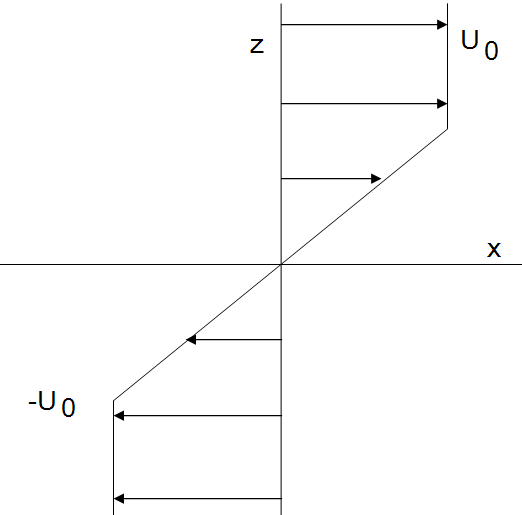
\includegraphics[width=0.9\textheight]{hopro.png}\\
  \caption{Velocity profile of a Holmboe mode}\label{hopro}
\end{figure}
